% This is samplepaper.tex, a sample chapter demonstrating the
% LLNCS macro package for Springer Computer Science proceedings;
% Version 2.21 of 2022/01/12
%
\documentclass[runningheads]{llncs}
%
\usepackage[T1]{fontenc}
% T1 fonts will be used to generate the final print and online PDFs,
% so please use T1 fonts in your manuscript whenever possible.
% Other font encondings may result in incorrect characters.
%
\usepackage{graphicx}
\usepackage{amsmath}
%\usepackage[citestyle=numeric-comp,]{biblatex}

\DeclareUnicodeCharacter{2212}{-}

% Used for displaying a sample figure. If possible, figure files should
% be included in EPS format.
%
% If you use the hyperref package, please uncomment the following two lines
% to display URLs in blue roman font according to Springer's eBook style:
%\usepackage{color}
%\renewcommand\UrlFont{\color{blue}\rmfamily}
%\urlstyle{rm}
%
\begin{document}
%
\title{Synchronization of chains of  logistic maps}
%
%\titlerunning{Abbreviated paper title}
% If the paper title is too long for the running head, you can set
% an abbreviated paper title here
%
\author{Franco Bagnoli \inst{1,2,\dagger}\orcidID{0000-0002-6293-0305} \and
Michele Baia\inst{1} \and
Tommaso Matteuzzi \inst{1} \and
Arkady Pikovsky\inst{3,\dagger}\orcidID{0000-0001-9682-7122}}
%
\authorrunning{F. Bagnoli et al.}
% First names are abbreviated in the running head.
% If there are more than two authors, 'et al.' is used.
%

% Affiliations / Addresses (Add [1] after \address if there is only one affiliation.)
\institute{Department of Physics and Astronomy and CSDC, University of Florence,  via G. Sansone 1, 50019 Sesto Fiorentino (Italy) \email{\{franco.bagnoli,michele.baia,tommaso.matteuzzi\}@unifi.it} \and INFN, Sect. Florence 
\and Institute of Physics and Astronomy, University of Potsdam, Karl-Liebknecht-Str. 24/25, 14476 Potsdam-Golm, Germany \email{pikovsky@uni-potsdam.de}}
%
\maketitle              % typeset the header of the contribution
%
\begin{abstract}
Master-slave synchronization can be exploited to ....

\keywords{Master-slave synchronization, data assimilation, parameter estimation.}
\end{abstract}
%
%
%
\section{Introduction}
Master-slave coupling consists in feeding part of master signal to a slave system~\cite{Pecora2015}, and can be considered as a completely asymmetric coupling in a one-dimensional lattice of chaotic elements. When the coupling ``strength'' is large enough, the two systems synchronize, provided they are using the same parameters, and, according with the type of coupling, there can be a relation between the maximum Lyapunov exponent of the unperturbed system (the master) and the critical strength for synchronization. 

Synchronization of chaotic systems has been a subject of extensive research since the 1990s, spurred by the seminal works of Pecora and Carroll ~\cite{Pecora1990}. Their pioneering demonstration of synchronization, achieved by compelling one system to emulate the dynamics of another, set the stage for numerous investigations in this field: from theoretical aspects, such as the relationship between synchronization and the nature of chaos~\cite{Gupte1993}, to more applicative ones.

Contrary to intuitive expectations, Maritan's discovery~\cite{Maritan1994} challenged the conventional belief that introducing randomness would exacerbate chaos. Further advancements by Ding and Ott~\cite{Ding1994} broadened the scope of synchronization methodologies, introducing a versatile transfer function capable of enforcing synchronization between systems with varying degrees of similarity. This newfound flexibility not only accommodated synchronization in non-identical systems but also facilitated synchronization under diverse timing conditions, ranging from continuous to discrete coupling ~\cite{Amritkar1993}\cite{Morgl1997}.

In parallel, the Active-Passive Decomposition (APD) method~\cite{Kocarev1995} introduced a novel perspective on synchronization, offering a robust framework for analyzing and achieving synchronization in chaotic dynamical systems. The potential applications of APD extend notably to secure transmission, where the preservation of signal quality remains paramount.

Beyond these foundational contributions, recent studies have pursued the generalization of synchronization principles. Investigations into phase synchronization~\cite{Rosenblum1996} and generalized synchronization with parameter mismatching [11] have expanded the theoretical repertoire, while explorations into spatiotemporal chaos have uncovered synchronization phenomena in a variety of complex systems, including coupled maps lattices~\cite{Jiang1998}, coupled systems exhibiting spatiotemporal chaos~\cite{Grassberger1999}, and Cellular Automata~\cite{Bagnoli1999}. Notably, these endeavors seek to establish connections between synchronization behaviors and universal classes such as directed percolation and the KPZ class ~\cite{Baroni2001} ~\cite{Droz2003}.\\

Master-slave synchronization can be quite useful for data assimilation, i.e., extracting the parameters of a model from a time series.
%~\cite{Bagnoli2023}. Let us first discuss the testbed case, in which the two systems are simulated in a computer. If the two systems use the same parameters, according with the type of coupling, there may be a critical value of the coupling strength above with the distance between them vanishes. If however the parameters are not the same, one in general has phase synchronization, for which, above the threshold, the two systems stay close. 
In Ref.~\cite{Bagnoli2023} we have shown that indeed one can exploit the fact that the complete synchronization occurs only for identical parameters to develop techniques for identifying the parameters of the master system, optimizing its distance from the slave one. This technique can be hopefully applied to experimental systems, coupling them to a simulated replica (assuming that one has a reliable model of the ``real'' system).\\

In the present work we investigate the problem of master-slave synchronization in chains of chaotic maps. We not only concentrate on the system formed by a master and a slave, but we consider also what happens to different slaves that receive the signal from the same master, and how slaves of slaves synchronize among them and with the master. 

%We examine the case of a chain of logistic maps , which exhibit a quite interesting synchronization pattern. 

After describing the general scheme in Section~\ref{sec:model}, we start studying the logistic map in Section~\ref{sec:logistic}, because it allows to put into evidence many aspects of the problem, in particular how a chain of masters and slaves synchronize. We shall show that there are quite unexpected phenomena, in particular that slaves synchronize among them for values of the coupling parameter much smaller that that required for the master-slave synchronization, and that this is related to the phenomenon of noise-induced synchronization \cite{Maritan1994}. 

%We then proceed applying the method to  continuous dynamical systems like Lorenz and Rössler ones. % (in Sections~\ref{sec:lorenz}. 

%We show that in most cases the synchronization pattern is quite different from that of the logistic map, and we shall related this difference to the sampling  of contracting and expanding regions  through the invariant measure induced by dynamics. 



\begin{figure}
    \centering
    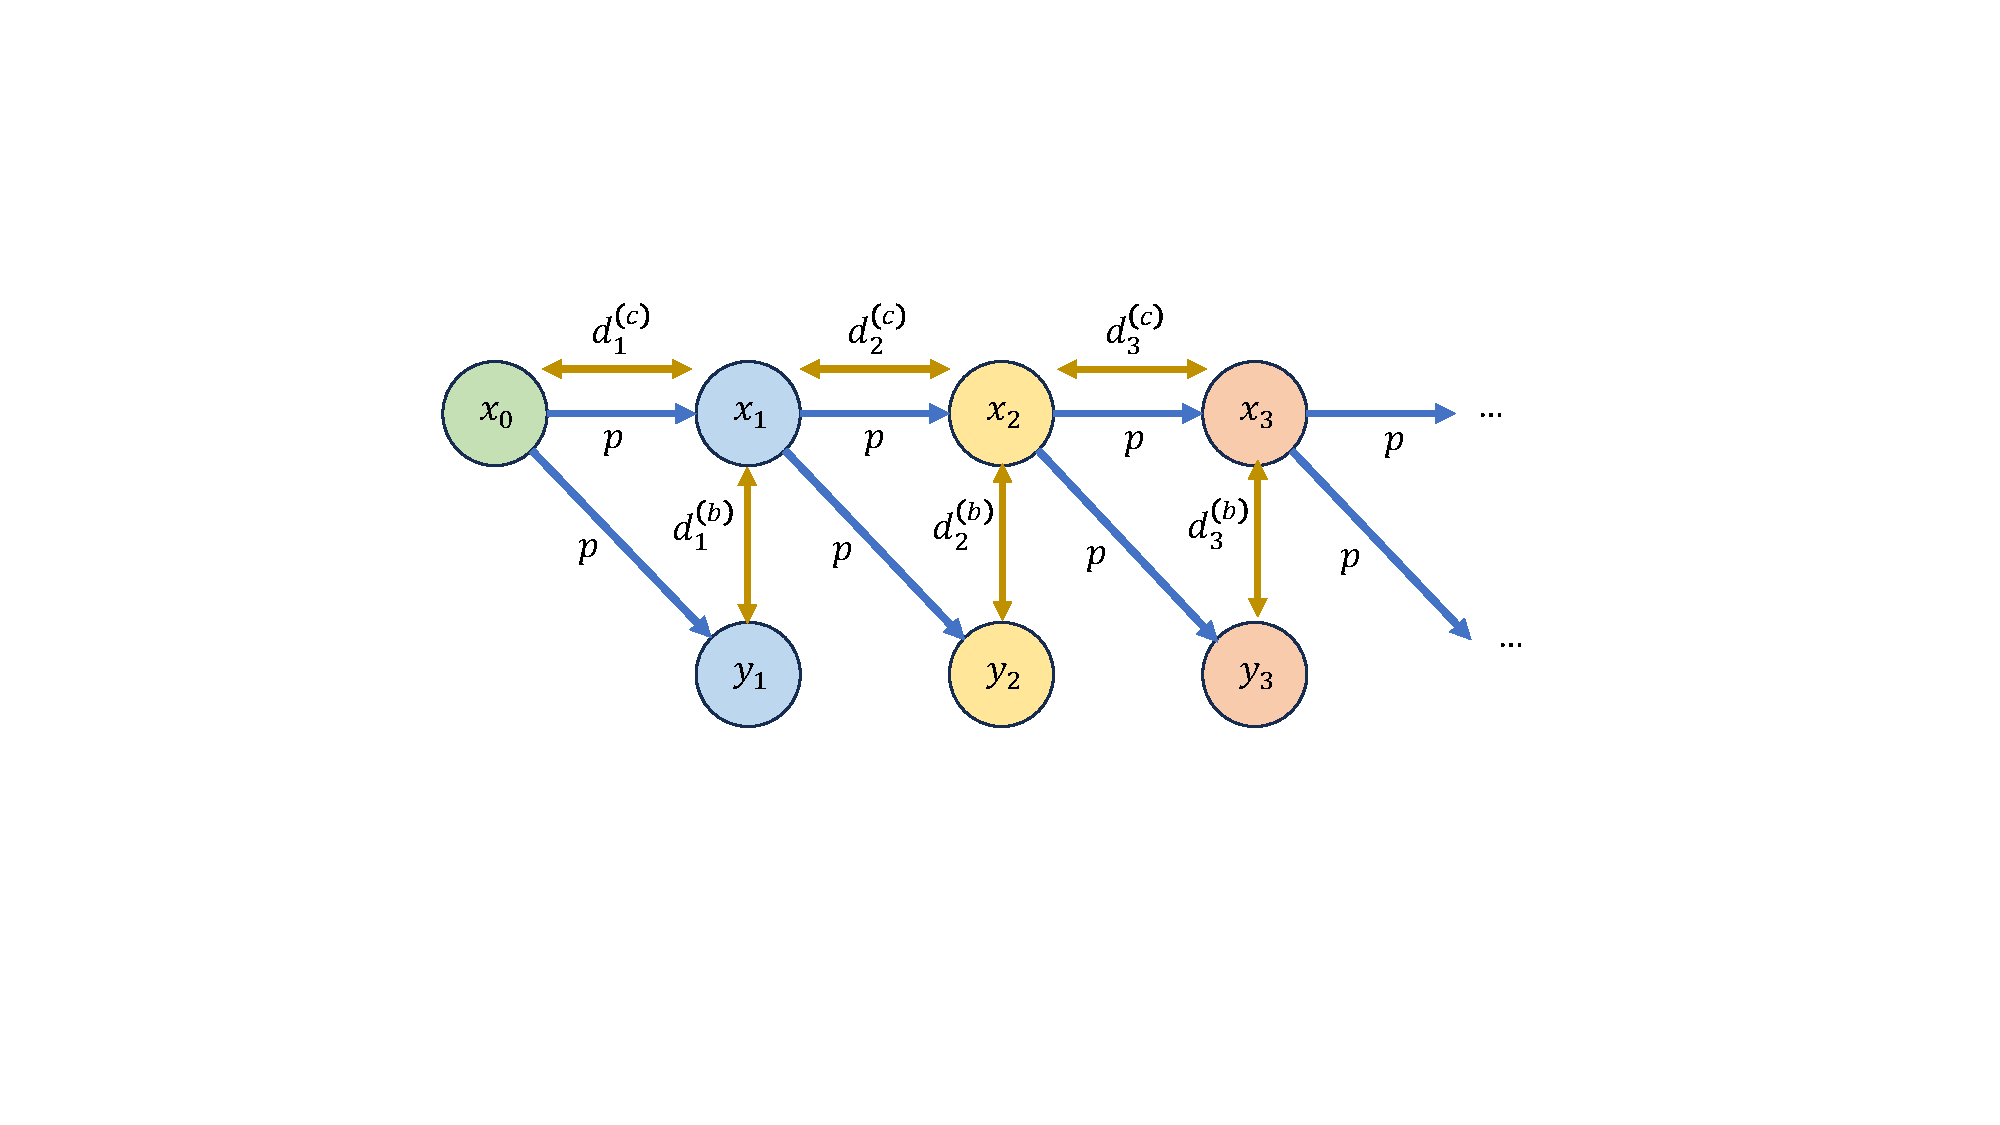
\includegraphics[width=0.7\linewidth]{CouplingScheme.pdf}
    \caption{The  coupling scheme among systems: $x_0$ denotes the master system. It has two "children", $x_1$ and $y_1$, and we measure the distance $d^{(1)}_c=\langle|x_0-x_1|\rangle$ between the master and one of its children, and  $d^{(1)}_b=\langle|x_1-y_1|\rangle$ between the two ``brothers''}
    \label{fig:CouplingScheme}
\end{figure}

\section{The chain model} \label{sec:model}
We consider one-dimensional maps, where the variable $r$ evolves in discrete steps, indexed by the time index $n$. In the following, we shall indicate by $r\equiv r(n)$ and $r'\equiv r(n+1)$. 

Let us consider a chain scheme, in which the first map evolves by itself 
\[
  r_0' = f(r_0),
\]
and all other maps evolve as 
\begin{equation}\label{eq:map}
  \begin{split}
    r_i' &= (1-p) f(r_i) + p f(r_{i-1});\\
    R_i' &= (1-p) f(R_i) + p f(R_{i-1}).\\
  \end{split}
\end{equation}
as shown in Fig.~\ref{fig:CouplingScheme}.

The $r_i$ are coupled as in the Pecora-Carrol scheme~\cite{Pecora1990,Pecora2015} (when applied to maps) with ``master'' $r_{i-1}$, while when we consider the difference between $r_i$ and $R_i$, these can be thought of as coupled by a ''noise'' term $r_{i-1}$. % as in the scheme presented in ~\cite{Maritan1994}.

We consider the differences
\begin{equation}\label{eq:delta}
  \begin{split}
    c_i &= \langle|r_i-r_{i-1}|\rangle;\\
    b_{i} &= \langle|R_i-r_i|\rangle;\\
  \end{split}
\end{equation}
and look for the synchronization thresholds $\pi_{i}^{(c)}: p |c_i=0$ and $\pi_i^{(b)}: p|b_i=0$. 

Near the synchronization thresholds, if the difference $\delta$ is small (and the transition is continuous), it is possible to linearly approximate the difference. We first denote by $\lambda_i$ the average 
\[
  \lambda_i = \frac{1}{N} \sum_{n=1}^N \ln\left(\left|\frac{\mathrm{d}{f}}{\mathrm{d}r}(r_i(n))\right|\right).
\]
Clearly, $\lambda_0$ is the Lyapunov exponent of the unperturbed  map. %(for the logistic map with  $a=4$, $\lambda_0=\ln(2) \simeq 0.693$). 

Let us derive the evolution equation for the difference of the first master-slave pair. 
\[
  c'_1 = |r'_1-r'_{0}| = (1-p) \left|f(r_1) - f(r_{0})\right|,
\]
Assuming $c'_1$ small, 
\[
f(r_{1})\simeq f(r_0) + \left(\frac{\mathrm{d}{f}}{\mathrm{d}r}(r_0)\right)(r_1-r_0), 
\]
\[
  c'_1 =  (1-p) \left|\frac{\mathrm{d}{f}}{\mathrm{d}r}(r_{0})\right|c_1.
\]
Therefore 
\[
  c_1(n) \simeq  \exp(\lambda^{(c)}_1 t)c_1(0),
\]
where 
\begin{equation}\label{eq:liapCteo}
\lambda^{(c)}_1 = \ln(1-p) + \frac{1}{T} \sum_t \ln\left(\left|\frac{\mathrm{d}{f}}{\mathrm{d}r}(r_{0}(t))\right|\right)= \ln(1-p) + \lambda_{0},
\end{equation}
and thus 
\begin{equation}\label{eq:pic}
\pi^{(c)}_1 = 1-\exp(-\lambda_0).
\end{equation}


This scheme does not work for the other master-slave pairs in the chain, since
\[
  \begin{split}
    r'_i &= (1-p) f(r_i) + p f(r_{i-1})\\
    r'_{i+1} &= (1-p) f(r_{i+1}) + p f(r_i))\\
  \end{split}
\]
and thus 
\[
  c_{i+1}(t) = \left|(1-p) (f(r_{i+1})-f(r_i)) + p (f(r_i)-f(r_{i-1}))\right|
\]
i.e., in the dynamics of the distance between maps $i+1$ and $i$ there is an explicit influence of map $i-1$, which acts as a kind of noise.    


On the other side, for the slave-slave pairs we have, 
\[
  b_i' = \left|R'_i-r'_{i}\right| = (1-p) \left|f(R_i) - f(r_{i})\right|,
\]
and again, assuming $\delta'^{(b)}_1$ small,
\[
f(R_{i})\simeq f(r_i) + \frac{\mathrm{d}{f}}{\mathrm{d}r}(r_i)(R_i-r_i),
\]
and thus
\[
  b'_i =  (1-p) \left|\frac{\mathrm{d}{f}}{\mathrm{d}r}(r_{i})\right|b_i,
\]
so  
\[
  b_i (t) \simeq  \exp(\lambda^{(b)}_i t)b_i(0),
\]
where 
\begin{equation}\label{eq:lambdab}
\lambda^{(b)}_i = \ln(1-p) + \frac{1}{N} \sum_{t=1}^N \ln\left(\left|\frac{\mathrm{d}{f}}{\mathrm{d}r}(r_{i}(n))\right|\right)= \ln(1-p) + \lambda_{i}.
\end{equation}

Clearly, also in this case the coupling with $r_{i-1}$ is present, but here it acts modifying the probability distribution of maps. 

Indeed, we can define the probability distribution of the single map $P_i(x)$ and compute the Lyapunov exponent $\lambda_i$ as
\begin{equation}\label{eq:lyapprob}
    \lambda_i = \int_0^1 \ln\left(\left|\frac{\mathrm{d}f}{\mathrm{d}r}(r)\right|\right) P(r)\mathrm{d}r.
\end{equation}

Notice that while $\pi^{(c)}_1$ depends on $\lambda_0$, i.e., the Lyapunov exponent of the unperturbed map, Eq.~\eqref{eq:pic}, $\pi^{(b)}_i$ (the value of $p$ such that $\lambda_i^{(b)}=0$) depends on $\lambda_i$, i.e., the Lyapunov exponent of the slave maps, Eq.~\eqref{eq:lambdab}.


\section{The logistic map}\label{sec:logistic}

The logistic map is defined by the recurrence equation 
\[
    r'=ar(1-r)
\]
and in the following we shall consider the case $a=4$, for which the asymptotic probability distribution of the state variable $r$ is $P(r) = 1/(\pi \sqrt(r(1-r)))$. The corresponding Lyapunov exponent is
\[
    \lambda_0 = \int_0^1 \frac{\ln(4|1-2x|)}{\pi \sqrt{r(1-r)}} \mathrm{d} r=\ln(2),
\]
and therefore
\[
    \pi^{(c)}_1=\frac{1}{2}.
\]
Indeed, we see from Fig.~\ref{fig:distlogistic} that the distance $c_1$ goes to zero for $p=0.5$. This transition is smooth. The other master-slave distances $c_i$ also goes to zero for $p=0.5$, but with a transition that is sharper and sharper, tending to a discontinuous transition for large values of $i$. We shall comment on it later. 

\begin{figure}
    \centering
    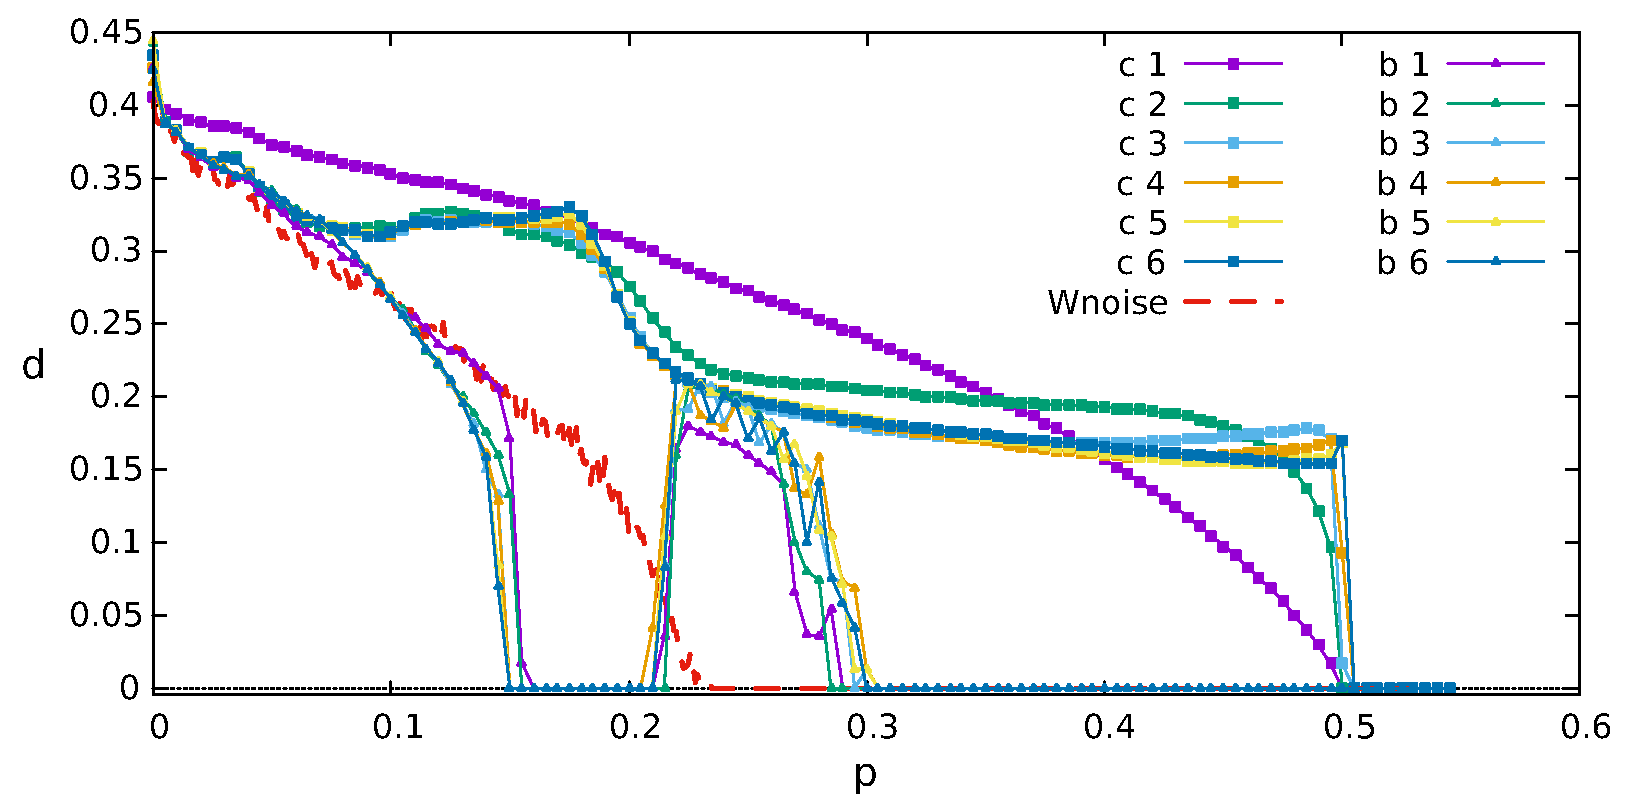
\includegraphics[width=0.35\textheight]{distancelogistic_b_c.pdf}
    \caption{The distances between master and slave and between the two slaves for the first $L=5$ layers of the logistic chain. Here $T=10^4$, TRANS$=10^5$, $R=100$, $a=4$. }
    \label{fig:distlogistic}
\end{figure}

\begin{figure}
    \centering
    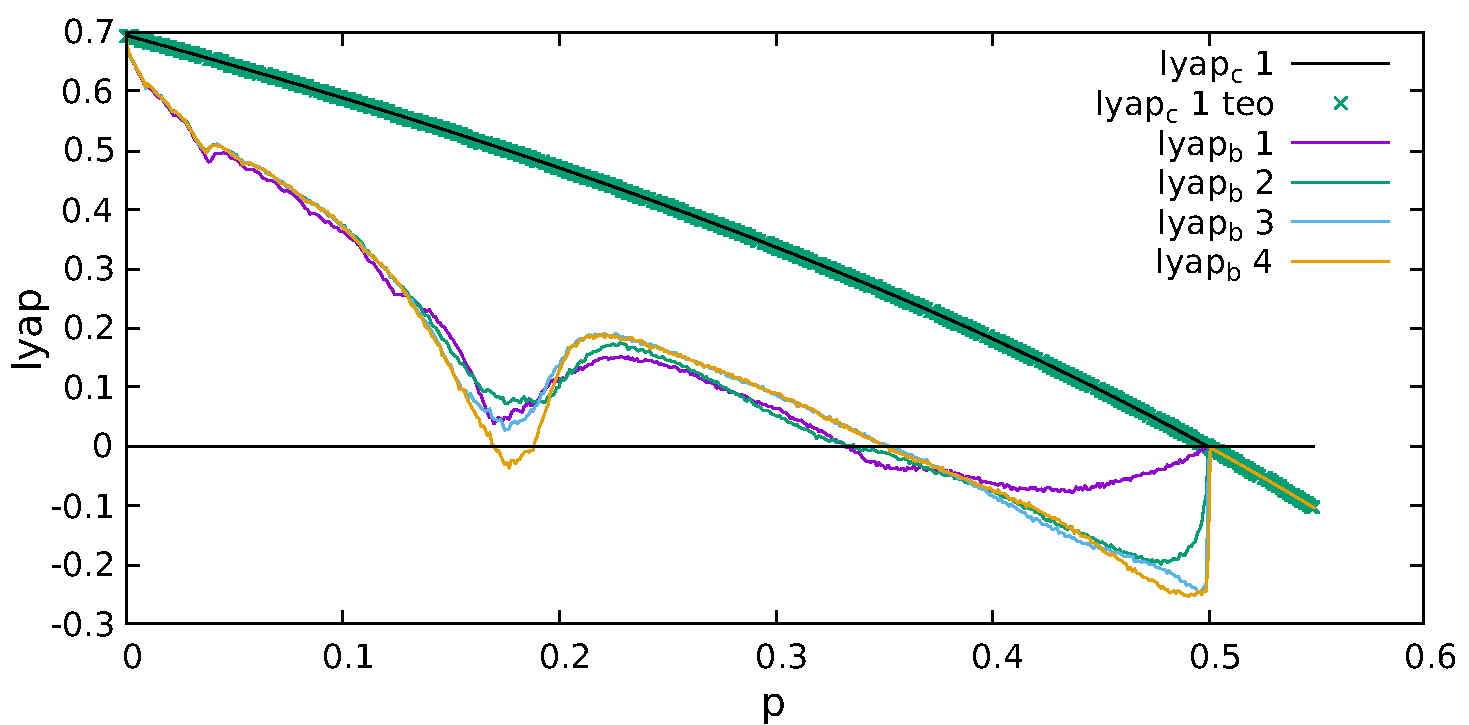
\includegraphics[width=0.5\textwidth]{logisticL5_lyap.pdf}
    \caption{The computed Lyapunov exponent $\lambda_1^{(c)}$ (\textit{$lyap_c 1$} in legend) and the Lyapunov exponent $\lambda_i^{(b)}$ of the chain. We also shoe the theoretical value of $\lambda^{(c)}_1$ (\textit{$lyap_c 1 teo$}) estimated using equation \ref{eq:liapCteo}. Here $T=10^4$, TRANS$=10^5$.}
    \label{fig:lambda-logistic}
\end{figure}

The slave-slave distances $b_i$ exhibit also a transition to zero for a value of $p$ around $0.32$, a value that can be estimated by evaluating $\lambda_i$, assuming that the values of $x_i$ and $x_{i-1}$ are uncorrelated since they are quite far from the master-slave synchronization transition, and that the action of $x_{i-1}$ is essentially that of an uncorrelated noise, all with similar probability distribution.

Indeed, we see from Fig.~\ref{fig:lambda-logistic} that all Lyapunov exponents $\lambda_i^b$ are essentially the same, before the synchronization transition. 

If we moreover assume a flat probability distribution of the master, $P(r)=1$, we get 
\[
    \lambda_i \simeq \int_0^1 \ln\left(4|1-2x|\right) dx = \ln(4)-1.
\]

We can therefore estimate the threshold $\pi_i^{(b)}$ for which $\lambda_1^{(b)}=0$
\[
    \pi_1^{(b)} = \frac{4-e}{4}\simeq 0.32,
\]
which is indeed near to the numerical results. 

The computed Lyapunov exponent for all slave maps becomes quite small for $p\in [0.16-0.2]$, but they are still positive (except for $\lambda_4$), but the slave maps exhibits a synchronization window around $p=0.2$, which becomes larger with the order index $i$, until growth saturates for $L>3$. In the correspondence of this synchronization window, the average master-slave distance increase, although the brother Lyapunov exponent of the single map, Fig.~\ref{fig:lambda-logistic} exhibit a decrease. 

In Figure \ref{fig:distlogistic}, we also display the average distance of two coupled logistic maps with white noise in $[0.0, 1.0]$ (red line).
We observe that the trend of the map coupled with white noise follows that of the brother distance in the chain, at least before the synchronization window around p=0.175, and, although shifted, even the way the two curves go to zero appears similar.
This made us reflect on the meaning and existence of this anomalous synchronization window.\\

\subsubsection{Synchronization and machine precision}.
Referring to Pikowsky's response to Martin and Banavar's article \cite{Maritan1994}, which points out that the synchronization of two coupled chaotic systems with white noise is essentially due to a machine precision error, we repeated the experiments with differently precision (from 32 bit up to 512 bit) to analyze the differences compared to previous simulations, obtained with double precision. 
In Figure \ref{fig:precision}(a), we present the brother-distance for the first node in the different cases. We also depict the behavior of the distance in the case of coupling with white noise computed with precision 32-bit and 512-bit. As can be observed, the trend of the brother-distance in the chain varies with precision. In particular, we observe that the increase in precision corresponds to a decrease in the width of the synchronization window observed in previous experiments, which disappears for precision greater than 128 bit. 

In Figure \ref{fig:precision}(b), we also show an example of the behavior of the brother distance in the first node for $p=0.17$. Specifically, we display the distance $b_1$ (in log10) in the case of low (64 bit) and high precision (512 bit). As evident, higher machine precision allows for a more accurate numerical representation, resulting in a difference in the last digits that leads to a minimum distance between the two nodes on the order of $10^{-25}$. For low machine precision synchronization is caused by an approximation error: at the given coupling parameter the distance eventually drop to value smaller that the machine precision.\\

\begin{figure}
    \centering
    \begin{tabular}{c c}
        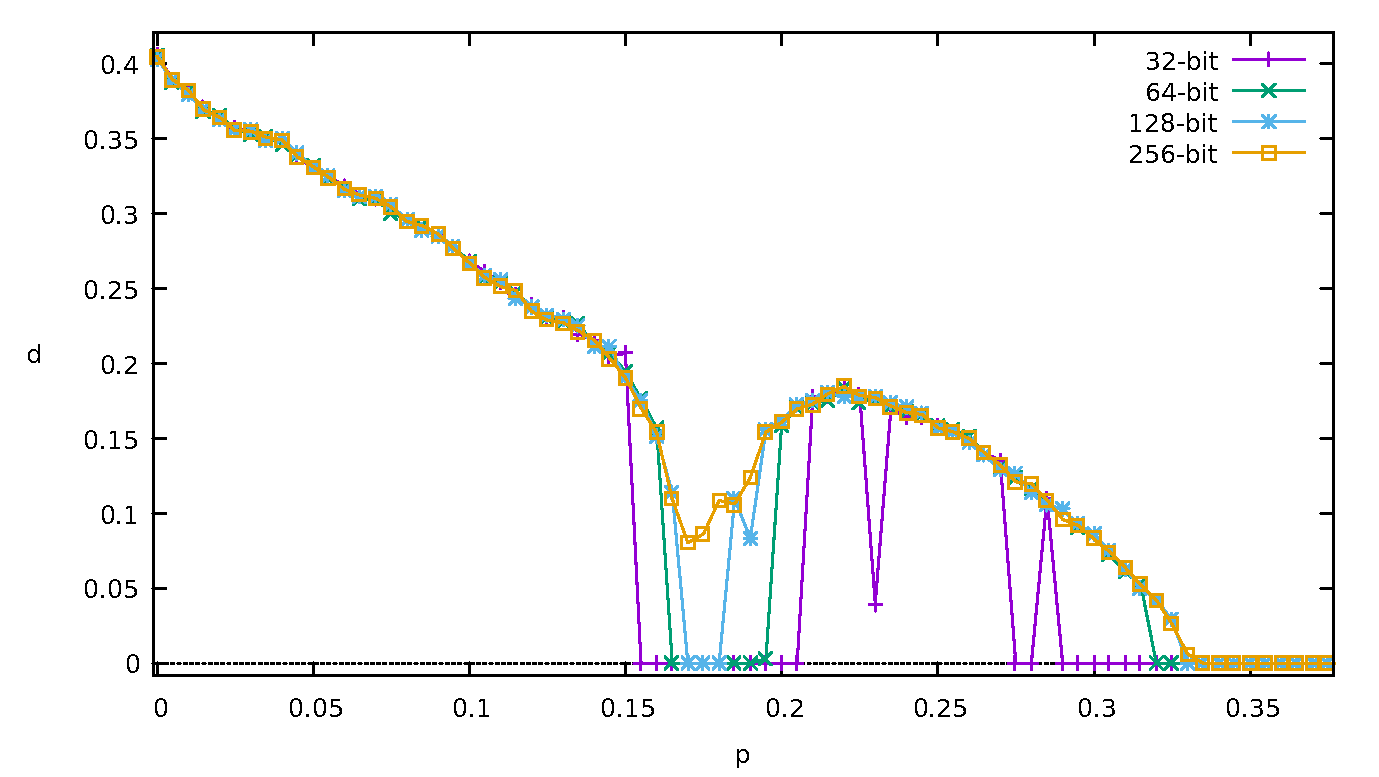
\includegraphics[width=0.45\textwidth]{distancelogistic_Precision.pdf} & 
        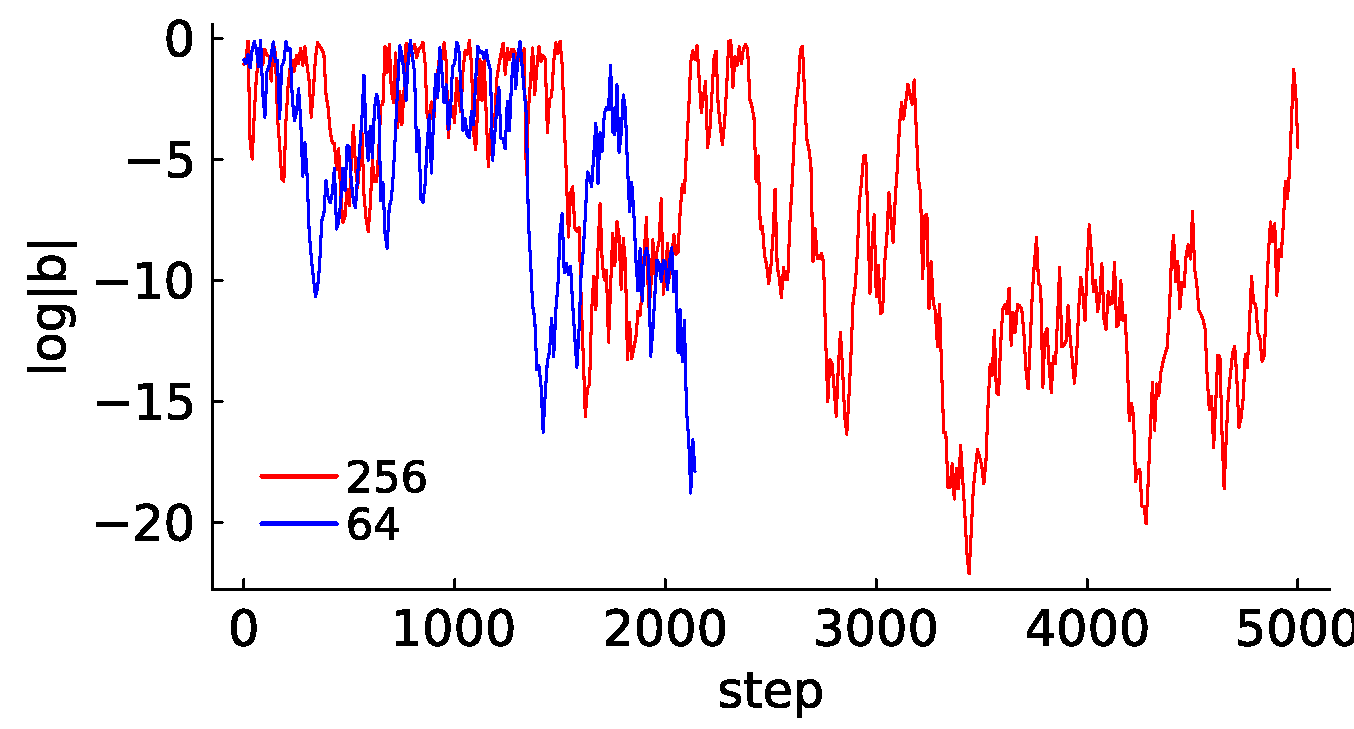
\includegraphics[width=0.45\textwidth]{logisticLogAbsDistanceBrother1.pdf} \\
         (a) & (b)  
    \end{tabular}
    \caption{(a) Brother distances of the first node computed with different machine precision (labeled as "$i$-bit", for $i = 32, 64, 128, 256$). Only for precision $\geq 256$ bit the synchronization window disappear. Here $T=10^4$, TRANS$=10^5$, $R=100$.
    (b) Plot of the time evolution of the brother distance of the first nodes ($\log_{10}b_1$) computed with 64 and 256-bit machine precision at coupling parameter $p=0.175$. Here $T=5000$.}
    \label{fig:precision}
\end{figure}


\subsubsection{Near the synchronization: $p \simeq \pi^c$}. 
To understand the behavior of global synchronization in Figure \ref{fig:logistic_distrib_chain} and \ref{fig:logistic_distance_evolution}, we show the probability distributions of maps in the chain and the temporal evolution of distances $c_1$ and $c_2$, which represent the distance between the master and the first child and between the first and second child, respectively, near the transition threshold $\pi^c$ in the case of a chain of logistic maps with L=10 layers. As observed in Figure \ref{fig:logistic_distance_evolution}, small perturbations in the distance between the first and second nodes propagate through the chain. This results in the probability distribution of the individual node being very different from that of the original logistic map. The deeper nodes, therefore, undergo a sharp transition to the synchronized state only when the preceding node has a probability distribution sufficiently similar to that of the decoupled map.

For finite simulation times, this phenomenon involves a natural shift of the transition threshold of the deep nodes of the chain (L>10). \\


\begin{figure}
    \centering
    \begin{tabular}{c c}
    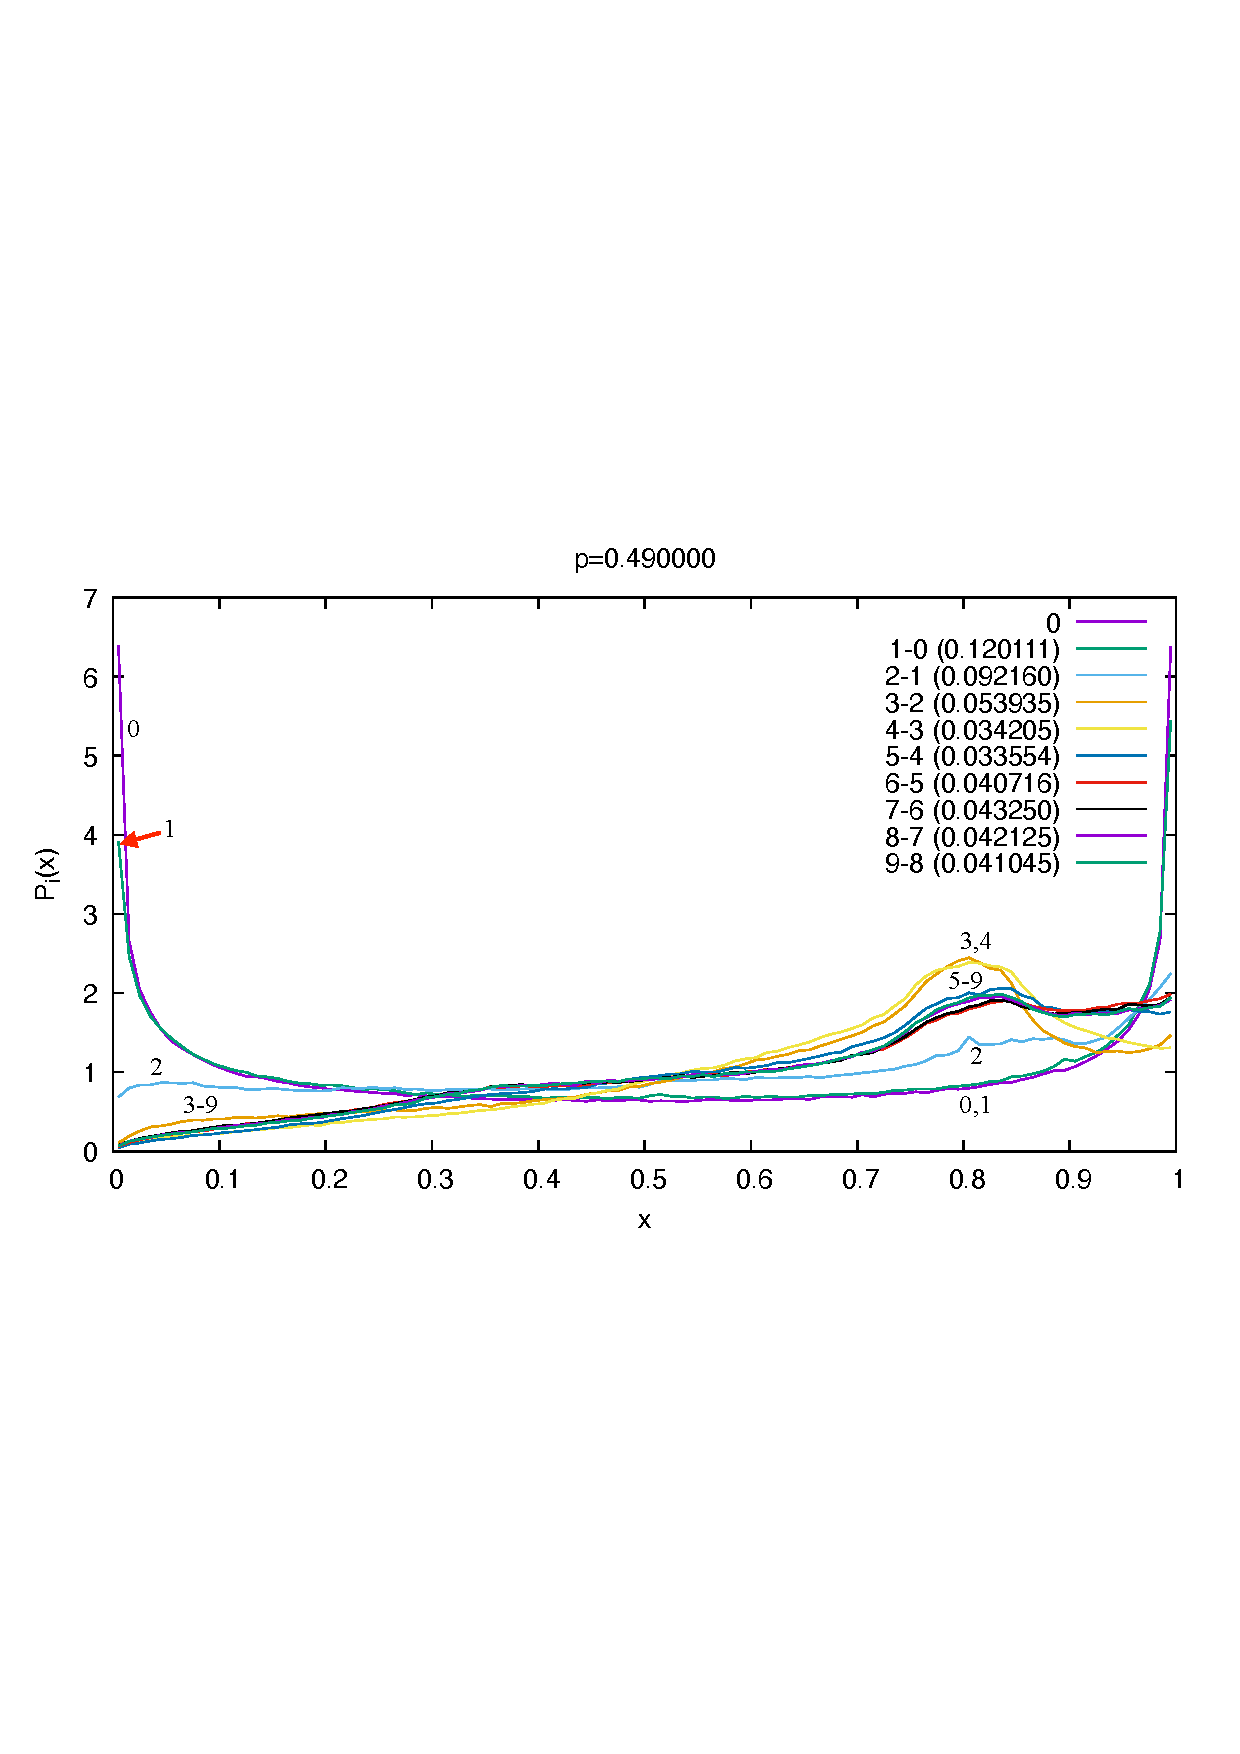
\includegraphics[width=0.45\textwidth]{logisticchain-distr-p=0.490.pdf} & 
     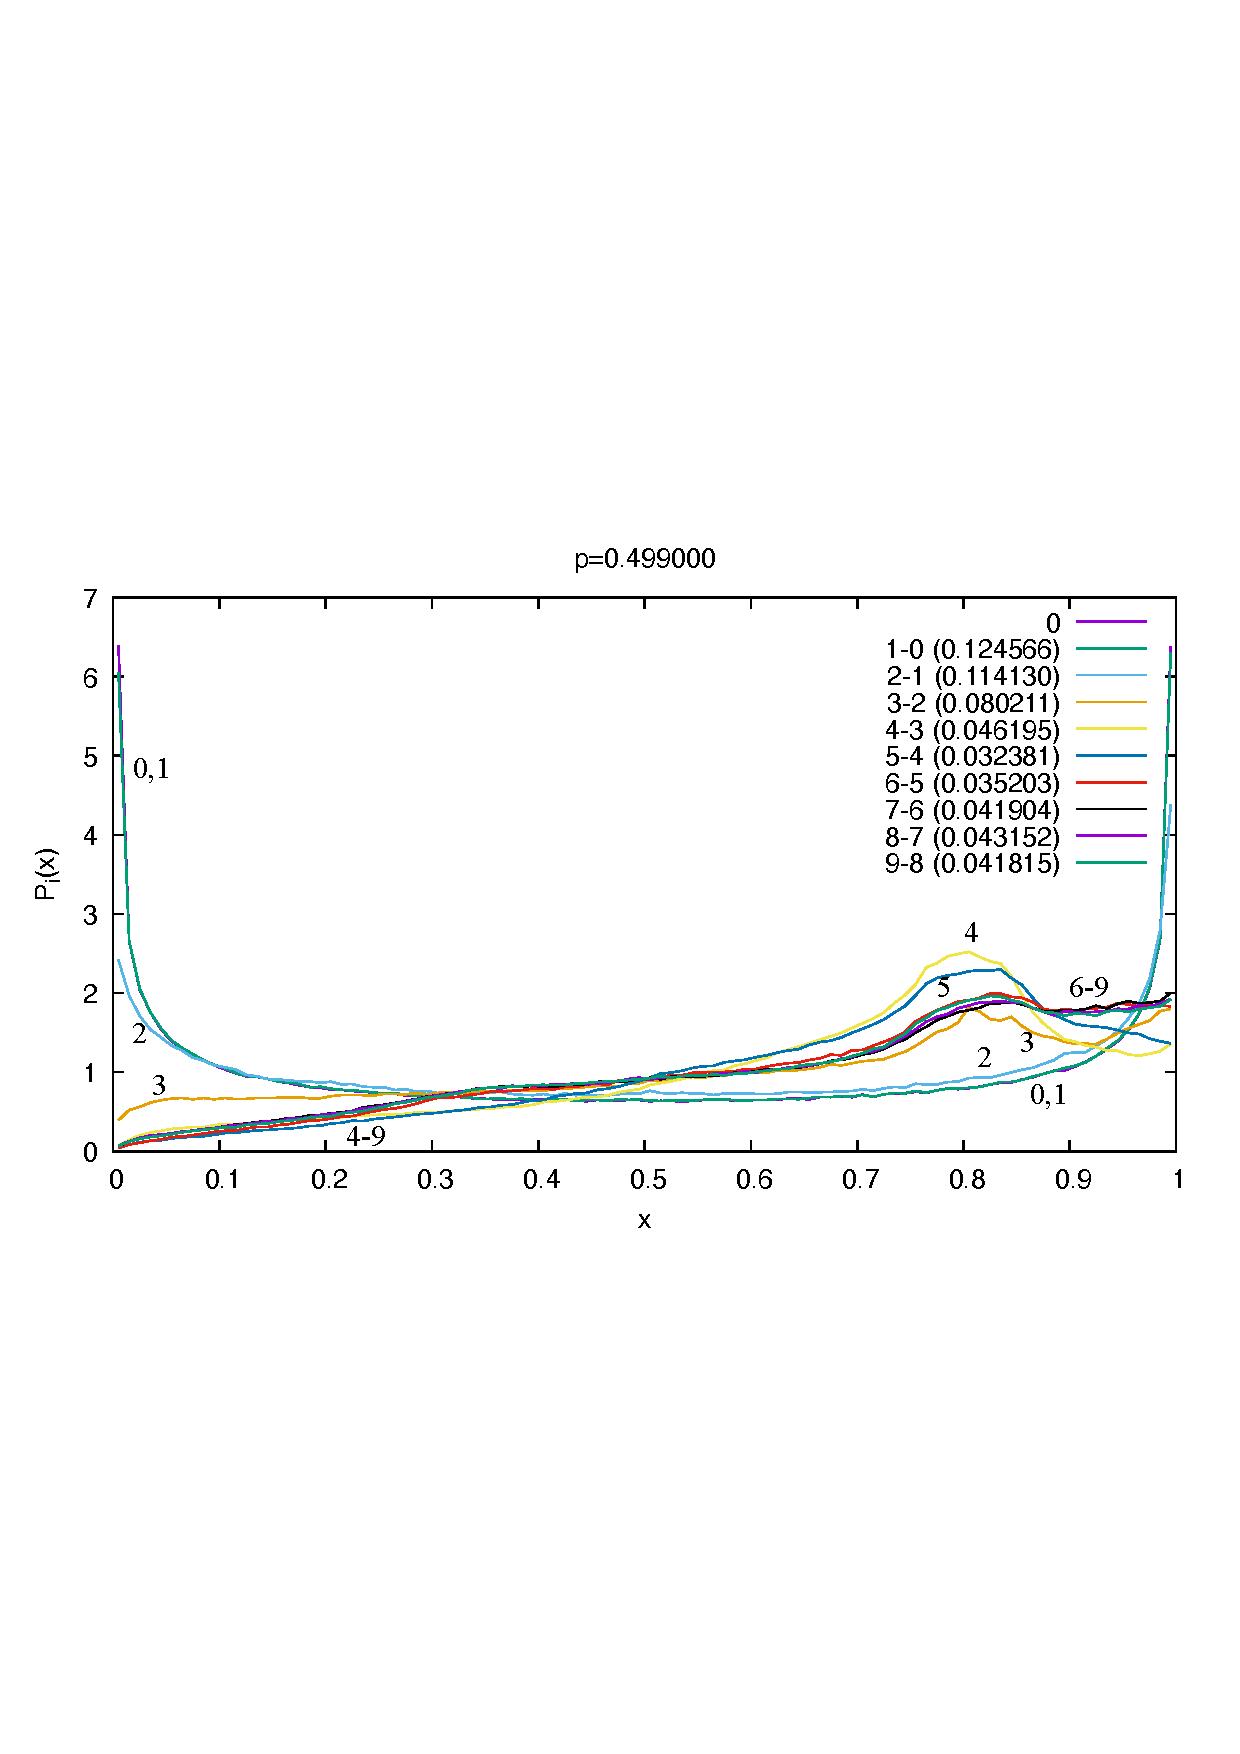
\includegraphics[width=0.45\textwidth]{logisticchain-distr-p=0.499.pdf}\\
     (a) & (b) \\
    \end{tabular}  
    \caption{Probability distribution of the maps in the chain. (a) $p=0.490$; (b) $p=0.499$. In parenthesis the correlation coefficient.}
    \label{fig:logistic_distrib_chain}   
\end{figure}

\begin{figure}
    \centering
    \begin{tabular}{cc}
    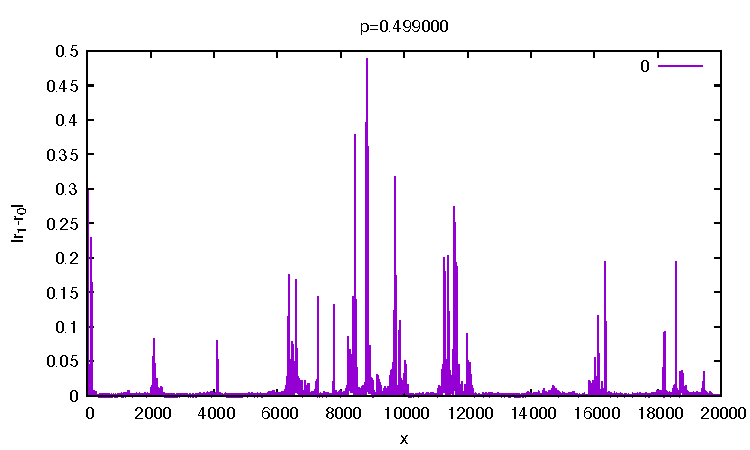
\includegraphics[width=0.45\textwidth]{logisticchain-temporal-10-p=0.499000.pdf} & 
     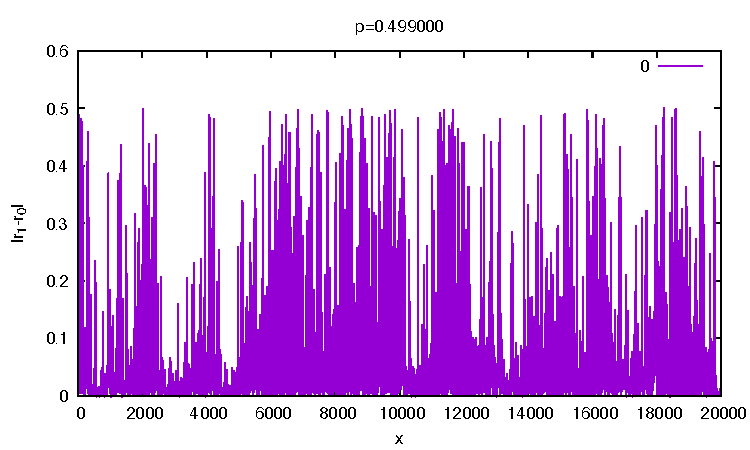
\includegraphics[width=0.45\textwidth]{logisticchain-temporal-21-p=0.499000.pdf}\\
     (a) & (b) \\
    \end{tabular}  
    \caption{Time evolution of the distance for $p=0.499$. (a) distance between maps 1 and 0; (b) distance between map 2 and 1. }
    \label{fig:logistic_distance_evolution}  
\end{figure}

\subsubsection{Synchronization of deeper nodes: $p > \pi^c$}.
The transition threshold shift, or more generally the propagation of noise in the chain, when the chain is in a syncronized state, can be studied by analyzing the time required for the network to absorb a disturbance from the globally synchronized state.

Let's assume we are in a condition of complete synchronization (p > $\pi_c$) and initialize the chain in a synchronized state (defined as the state in which all nodes of the chain have the same value as the master). We add noise to the initial condition of the first node and analyze the time required for individual nodes to return to the synchronized state. In Figure \ref{fig:logisticNoise_propagation} (a), we show, for different coupling values, the number of time steps required for the distance between the master and the i-th node $d^0_i = |x_i - x_0|$ to be zero in the case where a disturbance of intensity of the order of $\eta = 0.001$ is introduced into the initial condition of the first node. As observed, for depths up to L $\simeq 10$, the trend is approximately linear. The slope estimated from the data for different noise values as a function of the coupling parameter allows us to define a propagation velocity, or more accurately, a reabsorption velocity of the disturbance along the network. The trend of this velocity as a function of the coupling parameter can be explained using the definition of the velocity-dependent Lyapunov exponent $\lambda(v)$ given in \cite{Arkady93} such that: 

\begin{equation}\label{eq:lambdaVdep}
    \lambda(v) = \lambda_0 + c(y_0, v) + g(y_0, v),
\end{equation}

where $\lambda_0 = \ln 2$ is the Lyapunov exponent of the unperturbed map, and:
\begin{equation}
    \begin{split}
        y_0 &= 1 - v, \\
        g(y_0, v) &= (1−v) \ln (1 − p) + v \ln p, \\
        c(y_0, v) &= −(1−v) \ln (1 − v) − v \ln v. 
    \end{split}
\end{equation}

The reabsorption velocity $V$ can be estimated imposing $\lambda(V) = 0$. The simulation and the theoretical results are shown in Figure \ref{fig:logisticNoise_propagation} (b). 

%As observed, this value appears to be independent of the choice of noise introduced into the initial node. For values p $\gg \pi_c$, the relationship follows a power-law behavior: v $\propto$ p$^\alpha$, with $\alpha \simeq 4.95$ estimated experimentally.

For coupling values near the critical value $(\pi^c = 0.5$ for this system), this relationship no longer holds true due to numerical problem: the convergence time diverges even for the initial nodes, consequently, the velocity tends towards null values.  

% commenti:\\
%· Linear trend broken for L>10\\
%· to avoid early stopping, for the convergence time t: we choose t such that d[t:t+5] == 0!  


\begin{figure}
    \centering
    \begin{tabular}{c c}
    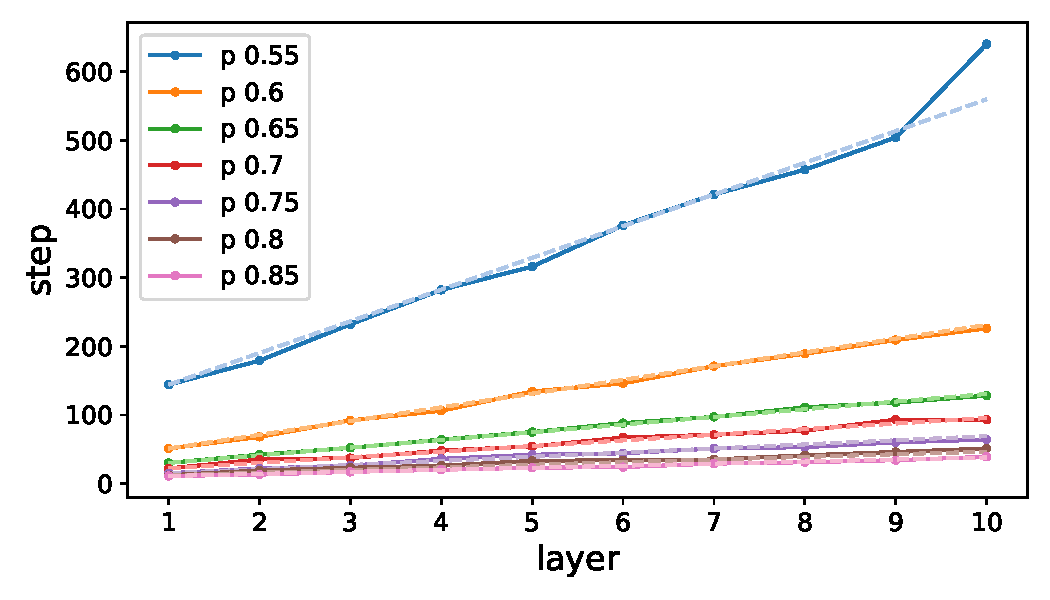
\includegraphics[width=0.45\textwidth]{logisticNoisePropagation_layerVsdeltaTimestep.pdf}  & 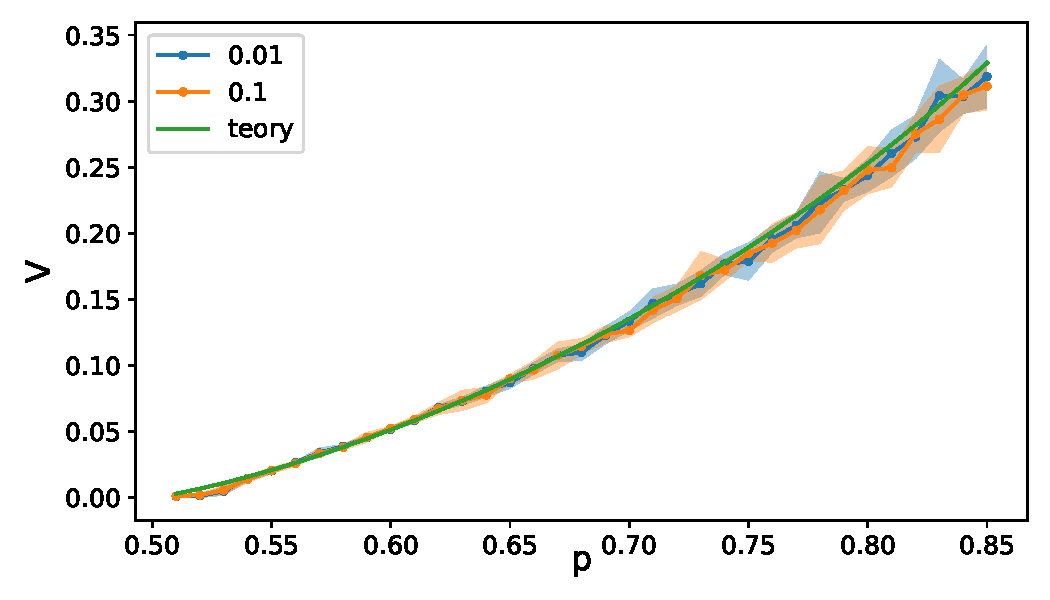
\includegraphics[width=0.45\textwidth]{logisticNoisePropagation_pVsVelocity.pdf} \\
        (a) & (b)
    \end{tabular}
    \caption{(a) Number of time step needed to reabsorb a perturbation of amplitude $\eta$ from a globally synchronized state. In dashed line the linear fit is shown. Here $L=20$ (only first ten showed), $T=10^3$, $\eta = 0.001$.
    (b) Velocity versus coupling parameter for different initial noise values $\eta$ (in legend) and theory result (eq.~\ref{eq:lambdaVdep}) for the logistics chain.}
    \label{fig:logisticNoise_propagation}
\end{figure}






%
% ---- Credits ----
%
\begin{credits}
\subsubsection{\ackname} acknowledgments.

\subsubsection{\discintname}
The authors declare no conflict of interest. The authors had no role in the collection of data from Wikipedia. (?)
\end{credits}
%
% ---- Bibliography ----
%
\bibliographystyle{splncs04}
\bibliography{synchro}


\end{document}
